\documentclass[tikz,border=2pt]{standalone}
\usepackage{amsmath,amssymb}
\usepackage{tikz}

\begin{document}
% Phone data with p = 6: y* = 22 sqrt(11/6) = 29.79, s* = 22 sqrt(6/11) = 16.25; stock phase
% s*/D = 8.1 days, shortage phase 6.8 days, cycle y*/D = 14.9 days.
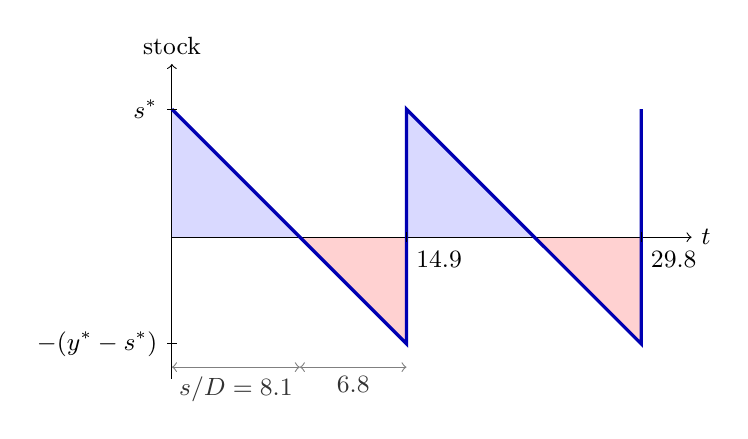
\begin{tikzpicture}[every node/.style={font=\small}, x=0.2cm, y=0.1cm]
	\fill[blue!15] (0,0) -- (0,16.25) -- (8.125,0) -- cycle;
	\fill[red!18] (8.125,0) -- (14.9,-13.54) -- (14.9,0) -- cycle;
	\fill[blue!15] (14.9,0) -- (14.9,16.25) -- (23.02,0) -- cycle;
	\fill[red!18] (23.02,0) -- (29.8,-13.54) -- (29.8,0) -- cycle;
	\draw[->] (0,0) -- (33,0) node[right] {$t$};
	\draw[->] (0,-18) -- (0,22) node[above] {stock};
	\draw[blue!70!black, very thick] (0,16.25) -- (14.9,-13.54) -- (14.9,16.25) -- (29.8,-13.54) -- (29.8,16.25);
	\draw (0.3,16.25) -- (-0.3,16.25) node[left] {$s^*$};
	\draw (0.3,-13.54) -- (-0.3,-13.54) node[left] {$-(y^*-s^*)$};
	\foreach \t/\l in {14.9/14.9, 29.8/29.8} {\draw (\t,0.6) -- (\t,-0.6) node[below right] {$\l$};}
	\draw[<->, gray] (0,-16.5) -- (8.125,-16.5) node[midway, below, text=gray!40!black] {$s/D=8.1$};
	\draw[<->, gray] (8.125,-16.5) -- (14.9,-16.5) node[midway, below, text=gray!40!black] {$6.8$};
\end{tikzpicture}
\end{document}
